

\begin{frame}{Empirical Orthogonal Functions}
    \section{Empirical Orthogonal Functions}
\begin{spacing}{1.5} 
\begin{itemize}
\item Statistical Tool:
\begin{itemize}
    \item One of the most used statistical analyses in atmospheric science.
    \item Also called Principal Component Analysis (PCA).
\end{itemize}
\item Properties:
\begin{itemize}
    \item Exploratory technique for multivariate data.
    \item Global analysis, misses localized phenomena.
    \item The choice of domain has large consequences, non-intrinsic.
    \item Might mix signals.
\end{itemize}
\end{itemize}
\end{spacing}
\end{frame}


\begin{frame}{Empirical Orthogonal Functions}
\begin{spacing}{1.5} 
\begin{itemize}
\item Correlation Matrix $\mathbf{C}$:
\begin{itemize}
    \item Its eigenvectors are spatial maps that capture how locations vary together.
    \item We look for the maps that explain the most variance in the data.
\end{itemize}
\item Eigenvalue Problem $\mathbf{C}\,\mathbf{e}_k = \lambda_k\,\mathbf{e}_k$:
\begin{itemize}
    \item Finding those maps reduces to solving an eigenvalue problem for $\mathbf{C}$.
    \item The largest eigenvalues $\lambda_k$ correspond to the dominant, most energetic patterns.
\end{itemize}
\end{itemize}
\end{spacing}
\end{frame}



\begin{frame}{Arctic Oscillation}
    \begin{figure}
          \centering
          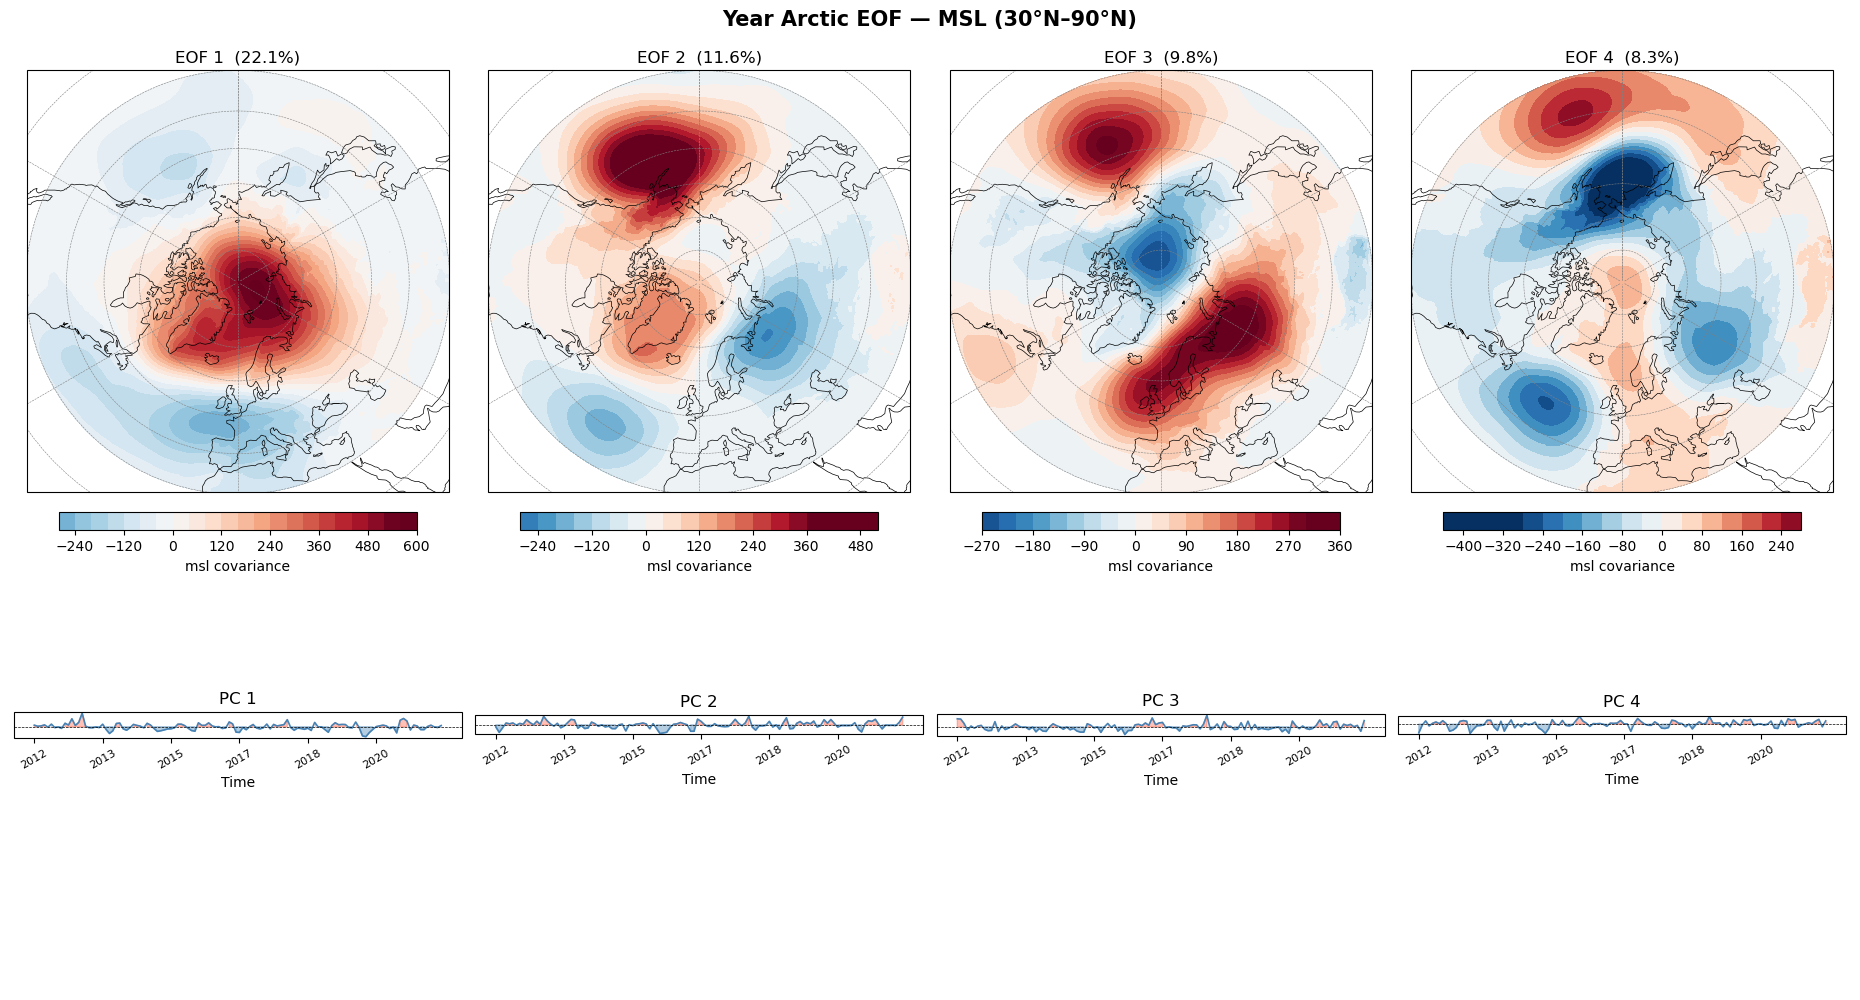
\includegraphics[height=0.6\textheight,keepaspectratio]{Figures/Year30MSL.png}
          \caption{Mean Sea Level Pressure}
    \end{figure}
\end{frame}

\begin{frame}{Winter Dipole Anomoly}
\begin{spacing}{1.5} 
\begin{itemize}
\item Trying to explain unexplained sea ice transport phenomena through the Fram Strait.
\item Importance of second leading EOF of MSLP in the arctic.
\item DA defined as this EOF.
\end{itemize}
\end{spacing}
\end{frame}

\begin{frame}{Dipole Anomaly}
    \begin{figure}
          \centering
          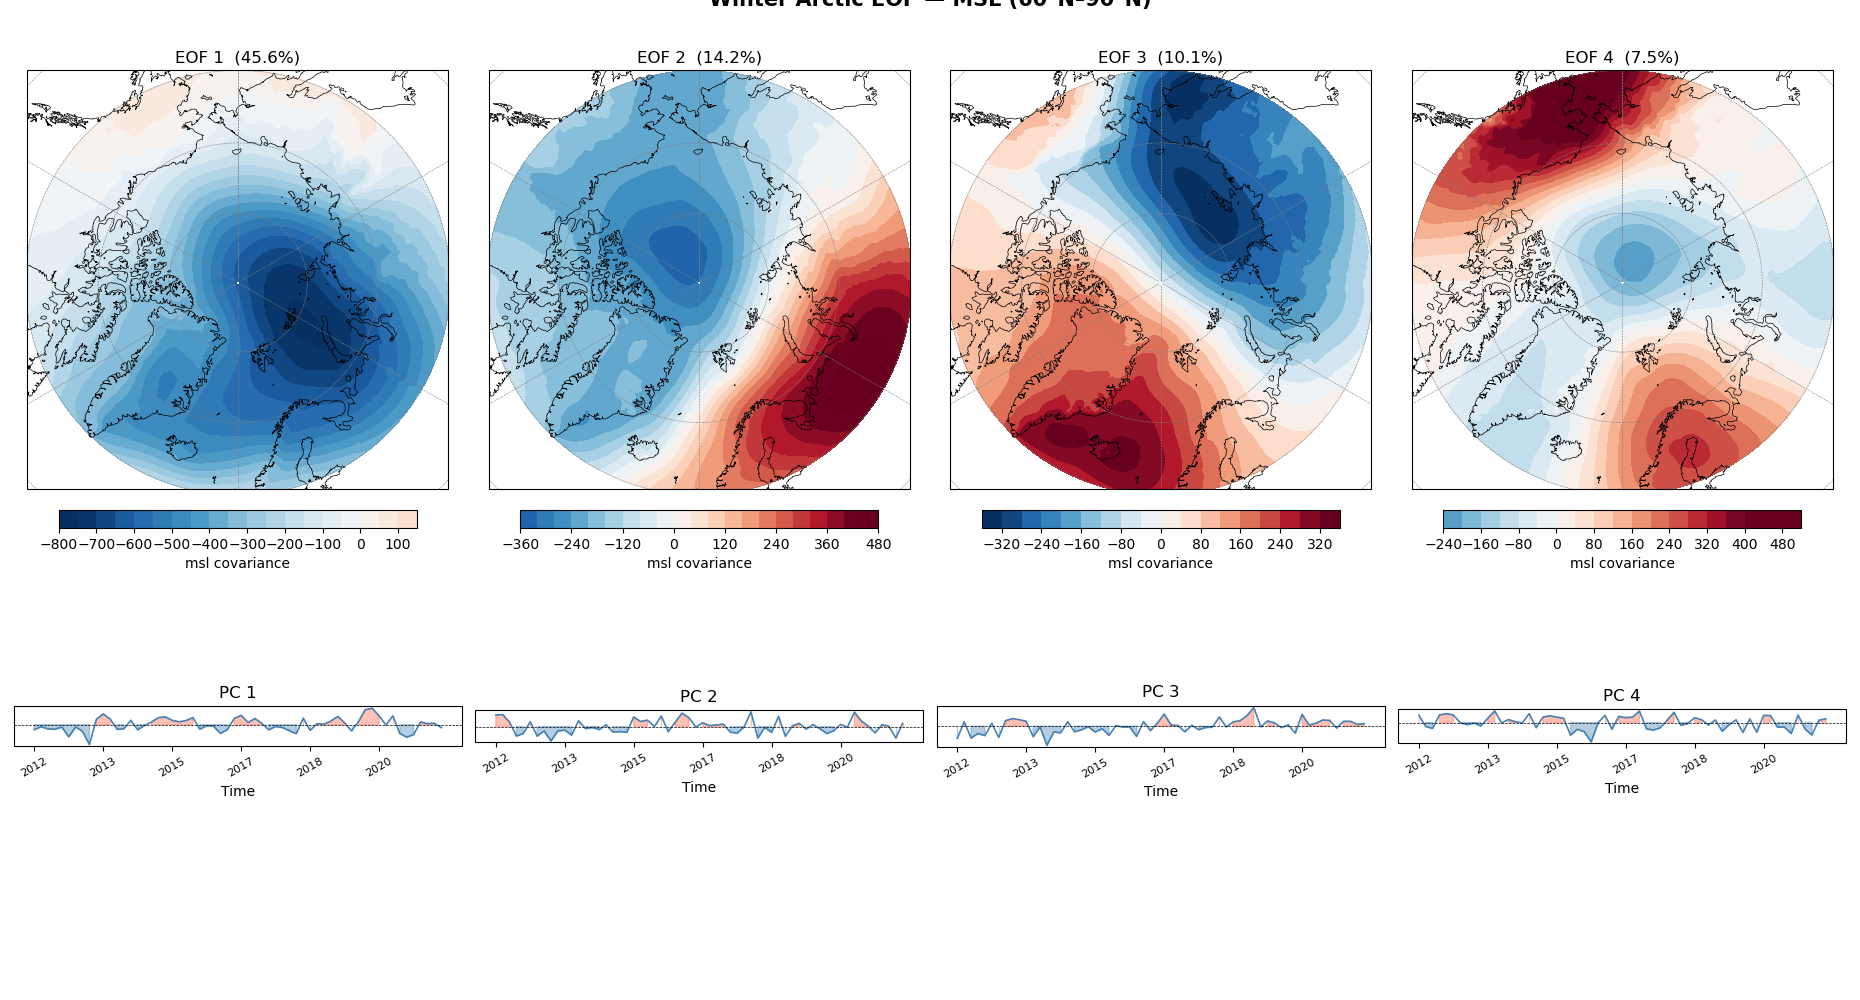
\includegraphics[height=0.6\textheight,keepaspectratio]{Figures/Winter60MSL.png}
          \caption{Mean Sea Level Pressure}
    \end{figure}
\end{frame}

\begin{frame}{T2M}
    \begin{figure}
          \centering
          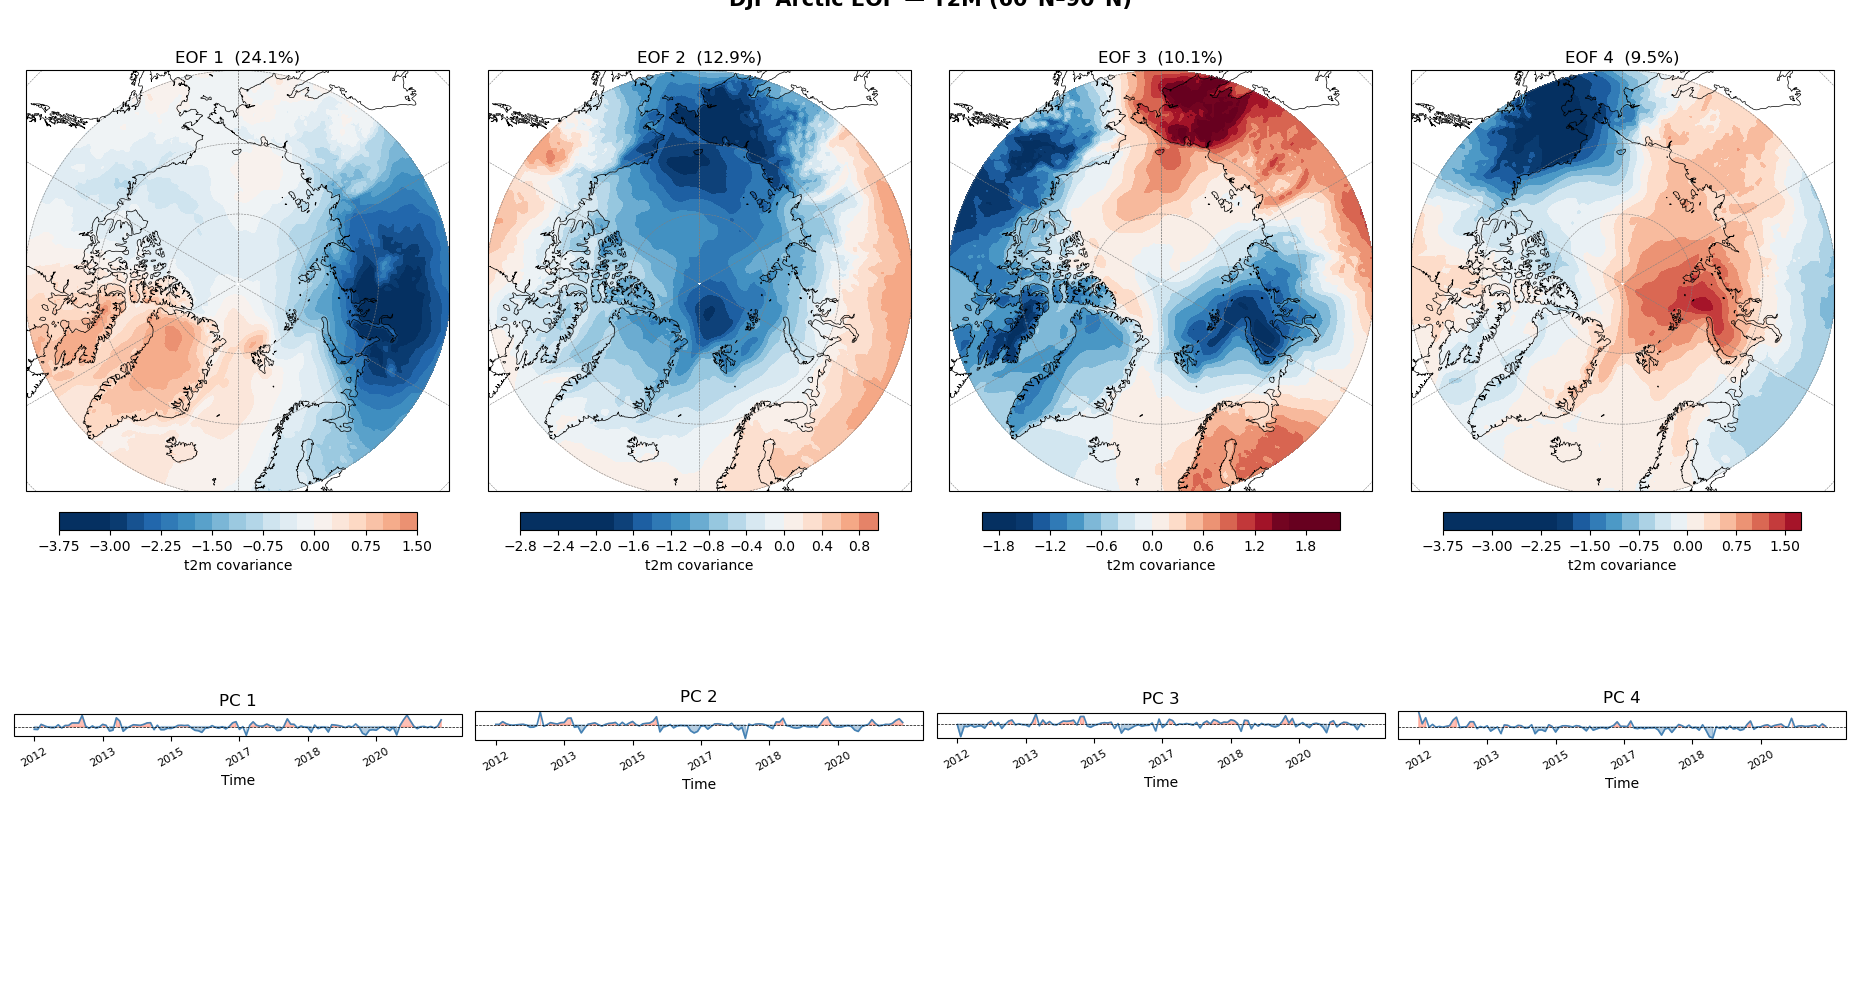
\includegraphics[height=0.6\textheight,keepaspectratio]{Figures/All60T2M.png}
          \caption{Temperaure at 2 Meters}
    \end{figure}
\end{frame}

\begin{frame}{SICONC}
    \begin{figure}
          \centering
          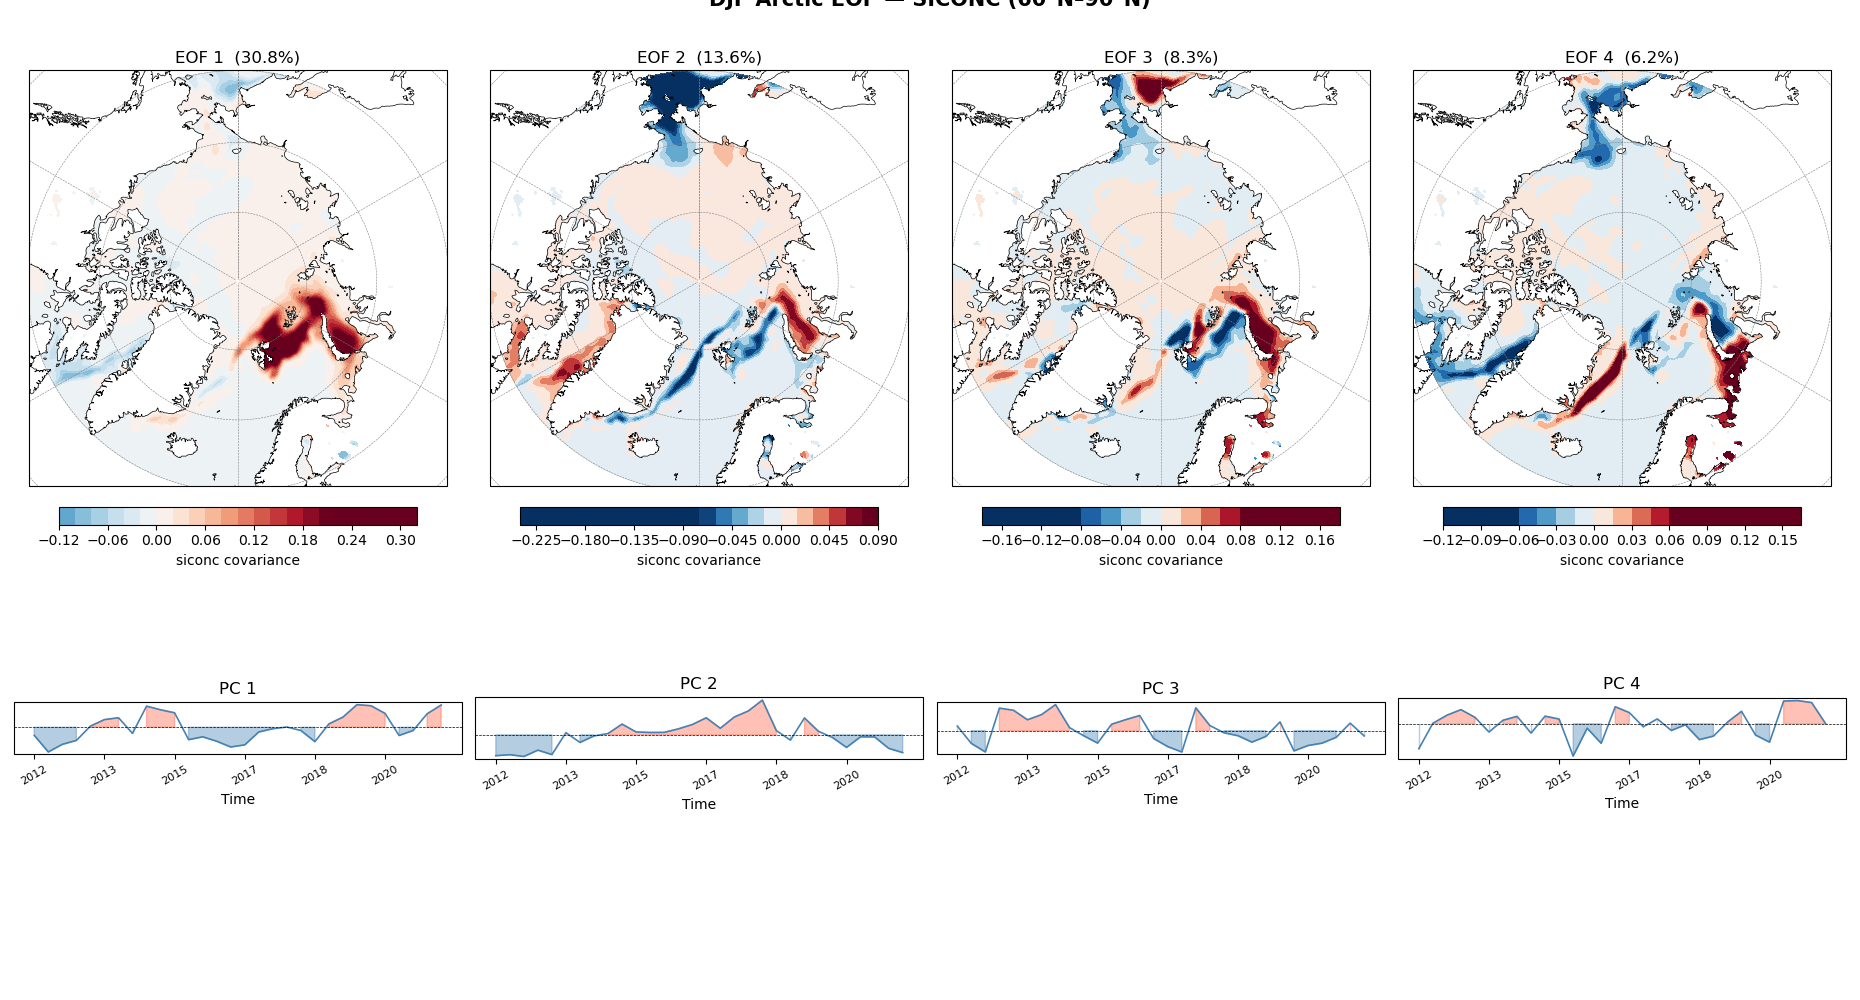
\includegraphics[height=0.6\textheight,keepaspectratio]{Figures/DJF60SICONC.png}
          \caption{Sea Ice Concentration}
    \end{figure}
\end{frame}